\documentclass{beamer}
\usepackage{movie15}
\usepackage{multirow}
\usepackage{amsmath}
\usepackage{amsthm}
\usepackage{amssymb}
\global\long\def\ev{\mathbb{E}}
\usetheme{metropolis}           % Use metropolis theme
\title{ A Kernel Test of Goodness of Fit}
\date{\today}
\author{Kacper Chwialkowski$^*$, Heiko Strathmann$^*$, Arthur Gretton}
\institute{}
\titlegraphic{
    %\includegraphics[width=2cm]{csml_logo_vector2.pdf}\hspace*{4.75cm}~%
   \includegraphics[width=2cm]{./img/csml_logo_vector2.pdf}
}
\begin{document}
\frame{\titlepage}
  \setbeamercolor{background canvas}{bg=white}
 \begin{frame}{What is one sample testing }
 \begin{center}
Are $\quad Z_i \sim p \quad$ where $\quad \log p \approx -|x|^{1.8} \quad$?\\
 \includegraphics[width=0.9\textwidth]{./img/mixtureOfNormal.pdf} 
 \end{center}
 
 \end{frame} 
  \begin{frame}{Building blocks}
\begin{center}
Kernel $k(x,t)$ and derivative of log density  $\partial_{x} \log p(x)$.
 \includegraphics[width=0.9\textwidth]{./img/kp.pdf} 
 \end{center}
 \end{frame} 
 
 
 \begin{frame}{Main idea}
We will use a cornerstone of modern ML.\\


\pause
\bf{Integration by parts.}
 \end{frame} 

  \begin{frame}{Cornerstone of modern ML: integration by parts}
\begin{align*}
 0= & \big( k(x,t) p(x) \big) \bigg |_{x=-\infty}^{x=\infty} \\
   = &  \int_{-\infty}^{\infty} \partial_{x} \big( k(x,t) p(x) \big)  dx \\
   = &  \int  \partial_{x} k(x,t) p(x)   + \big( \partial_{x} \log p(x) \big) p(x) k(x,t)  \\
   = &  \ev_p \partial_{x} k(X,t)   + \big( \partial_{x} \log p(X) \big)  k(X,t)\\
   = & \ev_p \xi_p(X,t)
\end{align*}

with $\xi_p(x,t) = \partial_{x} k(x,t)   + \big( \partial_{x} \log p(x) \big)  k(x,t)$
 \end{frame} 
  
 \begin{frame}{Cornerstone of modern ML cont}
$\xi_p(x,t) = \partial_{x} k(x,t)   + \big( \partial_{x} \log p(x) \big)  k(x,t)$ \\
$\ev_p \xi_p(X,t)=0$
 \includegraphics[width=0.9\textwidth]{./img/xi.pdf} 
 \end{frame} 
 
\begin{frame}{Main results I}
\begin{center}
If $X \sim p$ then $\ev_ p\xi_p(X,t)=0$
\\
\vspace{1cm}
If $Z \sim q \neq p$ then $\ev_q \xi_p(Z,t) \neq 0$
\end{center}
\end{frame} 

\begin{frame}{Main results II}
\begin{center}
$\ev_p \xi_p(X,\cdot)  \in \mathcal{H}_k$ \\ 
and \\
$\|\ev_p \xi_p(X,\cdot) \|_{\mathcal{H}_k}  = \ev_{p}h_p(X,X')$ \\
where 
\begin{align*}
h_{p}(x,y) & := \partial_{x} \log p(x) \partial_{x} \log p(y) k(x,y)\\
 & \quad+\partial_{y}\log p(y) \partial_{x}  k(x,y)\\
 & \quad+\partial_{x}\log p(x) \partial_{y}k(x,y)\\
 & \quad+\partial_{x} \partial_{y} k(x,y),
\end{align*}
\end{center}
\end{frame}

\begin{frame}{Function $h_p$}
\
 \begin{columns}
        \begin{column}{.5\textwidth}
        \vspace{1cm}
        \begin{figure}
%          \advance\leftskip-3cm
\advance\rightskip-2cm

           \includegraphics[width=\textwidth]{./img/h.pdf} 
        \end{figure}
        \end{column}
        \begin{column}{.5\textwidth}
        \vspace{-2cm}
           \begin{align*}
h_{p}(x,y) & := \partial_{x} \log p(x) \partial_{x} \log p(y) k(x,y)\\
 & \quad+\partial_{y}\log p(y) \partial_{x}  k(x,y)\\
 & \quad+\partial_{x}\log p(x) \partial_{y}k(x,y)\\
 & \quad+\partial_{x} \partial_{y} k(x,y),
\end{align*}
        \end{column}
    \end{columns}
 

 \end{frame}
 
 \begin{frame}{$V$-statistics}
An estimator of $\ev h_p(X,X')$ is
\[
 V_n(h_p) = \frac {1} {n^2} \sum_{i,j=1}^n h_p(X_i,X_j).
\]
Our test statistic is $ n V_n(h_p)$.

If $X_i \sim p$ then $ n V_n(h_p)$  converges weakly. 

Otherwise it does not,  it explodes, $P(n V_n(h_p) <C) \to 0$.
 \end{frame}
 
 
  \begin{frame}{$V$-statistics}
To estimate quantiles of $ V_n(h_p)$  
\[
 V_n(h_p) = \frac {1} {n^2} \sum_{i,j=1}^n h_p(X_i,X_j).
\]
under the null, we use wild bootstrap
\[
 B_n(h_p) = \frac {1} {n^2} \sum_{i,j=1}^n W_i W_j h_p(X_i,X_j).
\]
  where $W_i$ is a specific series of zero valued random variables.
\end{frame}

  \begin{frame}{Student's t vs.~Normal}
\begin{columns}
        \begin{column}{.5\textwidth}
        \begin{figure}
           \includegraphics[width=\textwidth]{img/sgld_student_bad} 
           
           
            \includegraphics[width=\textwidth]{img/sgld_student} 
        \end{figure}
        \end{column}
        \begin{column}{.5\textwidth}
            \begin{figure}
           \includegraphics[width=\textwidth]{img/sgld_student_opt} 
        \end{figure}
       Null -- samples are from normal distribution. Draws from the Student's t distribution exhibit temporal correlation.
        \end{column}
    \end{columns}
 

\end{frame}



  \begin{frame}{Bias quantification in Approximate MCMC}
\begin{columns}
        \begin{column}{.55\textwidth}
        \begin{figure}
           \includegraphics[width=\textwidth]{img/Heiko1} 
           
            \includegraphics[width=\textwidth]{img/Heiko2}
        \end{figure}
        \end{column}
        \begin{column}{.45\textwidth}
        \begin{align*}
\theta_{1}\sim{\cal N}(0,10);\theta_{2}\sim{\cal N}(0,1)\\
X_{i}\sim\frac{1}{2}{\cal N}(\theta_{1},4)+\frac{1}{2}{\cal N}(\theta_{2},4) & .
\end{align*}

            \begin{figure}
           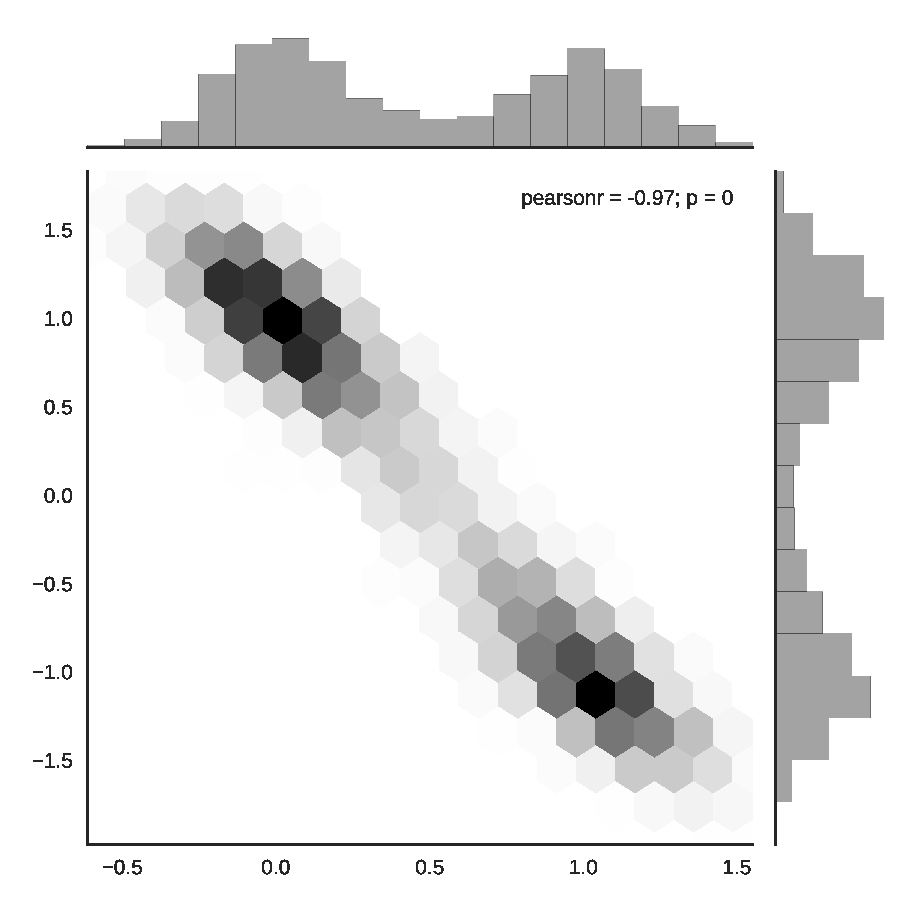
\includegraphics[width=\textwidth]{img/sgld_sample} 
        \end{figure}

        \end{column}
    \end{columns}
 \end{frame}

  \begin{frame}{Experiment 3}
\begin{columns}
        \begin{column}{.5\textwidth}
        \begin{figure}
           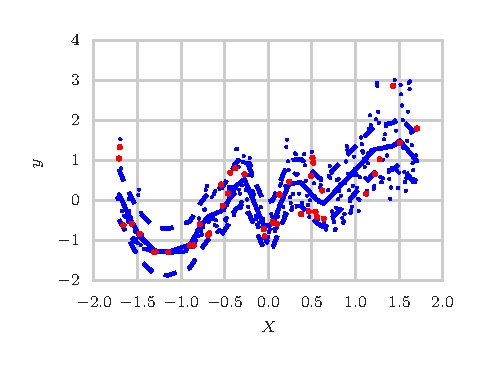
\includegraphics[width=\textwidth]{img/gp_regression_data_fit} 
             
             \includegraphics[width=\textwidth]{img/gp_regression_bootstrap_hist} 
        \end{figure}
        \end{column}
        \begin{column}{.5\textwidth}
       We use the \texttt{solar} dataset. We fit $N_{\text{train}}=361$
data using a GP, and perform  maximum likelihood. We then apply our test
to the remaining $N_{\text{test}}=41$ data.
        \end{column}
    \end{columns}
 
 \end{frame}


\end{document}